\documentclass{article}
\usepackage[letterpaper, margin=1in]{geometry}
\usepackage{amssymb}
\usepackage{amsmath}
\usepackage{graphicx}

\topmargin = -70pt

\title{HW 2}
\author{Yunhao Lin}

\begin{document}
\maketitle
\section{Part A:}
\begin{enumerate}
\item    If both \textit{a} and \textit{b} are concave, and from the Problem 
 description, we know both sequence of \textit{a} and sequences of \textit{b} 
 are all non-decreasing sequence. Therefore,$z_i = a_i + b_{k-i}$, and $z_{i+1}
 = a_{i+1} + b_{k-(i+1)}$, $z_{i-1} = a_{i-1} + b_{k-(i-1)}$. In order to prove
 $z_i$ is a concave function as a function of $i$. From the definition of concave,
 if $z_i - z_{i-1} \geq z_{i+1} - z_i$, then $z_i$ is concave.\\
 Therefore, $z_i - z_{i-1} = (a_i + b_{k-i})-(a_{i-1} + b_{k-i+1}) = (a_i - a_{i-1}) + 
 (b_{k-i} - b_{k-i+1})$ and $z_{i+1} - z_i = (a_{i+1}+b_{k-i-1}) - (a_i + b_{k-i}) 
 = (a_{i+1} - a_i) + (b_{k-i-1} - b_{k-i})$. Because sequence a is a non-decreasing
 concave sequence, it follows the definition that states: $a_i - a_{i-1} \geq 
 a_{i+i} - a_i$. Assume $ k - i = x $, and because sequence b is also a 
 non-decreasing concave sequence, from the description: $b_x - b_{x-1} \geq 
 b_{x+1}-b_x$. Add the $b_{x-1}$ on both side and subtract $b_{x+1}$ on both 
 side would result in $b_x - b_{x+1} \geq b_{x-1}-b_x$.
 $\because a_i - a_{i-1} \geq a_{i+i} - a_i $ \\
 $\because b_x - b_{x+1} \geq b_{x-1}-b_x \Rightarrow b_{k-i} -b_{k-i+1} \geq 
 b_{k-i-1} - b_{k-i}$\\$\therefore $ add the previous two equation $(a_i - a_{i-1}) 
 + (b_{k-i} - b_{k-i+1} \geq (a_{i+1} - a_i)+ (b_{k-i-1} - b_{k-i})$\\
 $\therefore (a_i + b_{k-i})-(a_{i-1} + b_{k-i+1}) \geq (a_{i+1}+b_{k-i-1}) - 
 (a_i + b_{k-i})$\\ $\therefore z_i - z_{i-1} \geq z_{i+1} - z_i$ \\
 Therefore by definition, the sequence $z_i = a_i +b_{k-i}$ is also concave function as i.

 \item  In order to find $c_k$, by the definition of $c_k$, we need to find 
 the largest value of $a_i + b_{k-i}$ which as 1 indicates, is the largest 
 value in the sequence \textit{z}. 
 Assuming both sequence \textit{a} and sequence \textit{b} is concave, then 
 as proved in Part A: 1, sequence \textit{z} is also concave. \\First, we need 
 to find the middle element of sequence \textit{z} at index [$\frac{k}{2}$], 
 name it $z_a$. Then compare $z_a$ with two element next to itself. Name the element
  at index [$\frac{k}{2}-1$], $z_l$ and the element at index [$\frac{n}{2}+1$]
 ,$z_r$. If $z_a$ is the largest of the three or $z_a$ is equal to either $z_i$ 
 or $z_r$, return $z_a$ to be the largest element in the sequence. If $z_a$ is not 
 the largest of the three, but $z_l$ is the largest. The maximum number
 of the whole sequence must be located on the left half. Otherwise $z_r$ is 
 the largest of the three, the maximum number would locate on the right half of 
 the sequence. \\
 Therefore, we recurse on the left half or the right half of the sequence. 
 Since there are two calls to the subproblems(right part of the sequence and 
 left part of the sequence), we have two T($\frac{k}{2}$)
 but we are executing on side on each recursive call. We also have to check 
 if $z_l$ is the largest element or equal to $z_l$ or $z_r$, that takes 
 constant O(1) time. So, the runtime is T(n) =  T($\frac{k}{2}$) + O(1) = O($\log_{2} k$).\\\\
 \textit{Proof:} \\
 \textbf{Base Case:} When k = 2, There are only 2 $c_k$, $z_a$ is at index 1 and
 there is no element on the left, which means there is no $z_l$, we just need to 
 compare it with the $z_r$ and return the larger one to be $c_k$.\\
 \textbf{Other cases:} Since z is a concave sequence, the slope of z is non-increasing
 over time. So when we choose the middle point of the whole sequence z --- $z_a$. 
 If one of $z_l$ and $z_r$ or both are equal to $z_a$, then the slope at $z_a$ is 
 equal to 0, and as we already know the slope is non-increasing, there cannot be any 
 value larger than $z_a$. Therefore, $z_a$ is the largest element in the sequence and
  we return $z_a$. If none of $z_l$ and $z_r$ is equal to $z_a$. 
 There is two conditions:
 \begin{itemize}
     \item If both $z_l$ and $z_r$ are smaller than $z_a$, since the slope is non-increasing, $z-a$ 
     is the point for the slope to turn from positive to negative. Otherwise, $z_a$ and $z_r$ cannot
     be both smaller than $z_a$. Because $z_i$ is a concave function, slope is decreasing on the left
     side of $z_a$ but are all positive, every point before $z_l$ cannot be larger than $z_l$. 
     Slope on the right side of $z_a$ is decreasing and negative, therefore every point beyond $z_r$ 
     cannot be larger than $z_r$. Therefore, we return $z_a$ as the largest value of the whole sequence.
     \item If one of $z_l$ and $z_r$ is smaller and one is larger, we just take the part where has the 
     larger part. Since the concave function suggests that the slope before is non-increasing and the
     slope after is non-increasing. Either way is going to yield a result that elements on one side 
     is larger than all the element on the other side. So we choose the side with the larger value and 
     call recursive function on that side. 
 \end{itemize}
\end{enumerate}

\section{Part B:}
\begin{enumerate}
\setcounter{enumi}{3}
\item As we know i(k) is the largest index that maximizes the sum $a_i + b_{k-i}$, let the index
be indicated by $i_k$. We now know $a_{i_k} + b_{k-i_k}$ is the biggest for every $i$. \\
\\\textit{Proof:} Assume that i(k) is decreasing as a function of $k$, i.e. $i(k) > i(k+1)$.\\
This statement means that there is a i(k+1) that is smaller than i(k). We are going to name the 
index i(k+i) as ($i_k-l$), l is some constant number that is smaller than $i_k$ 
so that $i_k-l > 0$. Therefore, there exist $a_{i_k-l} + b_{k+1-i_k+l}$ that marks the 
largest value of sum $a_i + b_{k+1-i}$. 
Because i(k) is the largest index, i(k) is larger than any other index:
\begin{align}
    \because a_{i_k} + b_{k-i_k} \geq a_{i_k-l} + b_{k-i_k+l}
\end{align}
When there is k+1 elements, in order for i(k+1) to be smaller than i(k). We are using
$>$ sign here because in order to choose the largest index, if $a_{i_k-l} + b_{k+1-i_k+l}
 = a_{i_k} + b_{k-i_k+l}$, it would choose the $i(k)$ term rather than i(k+1):
\begin{align}
    a_{i_k-l} + b_{k+1-i_k+l} > a_{i_k} + b_{k-i_k+l}
\end{align}

Because the sequence of b is concave and non decreasing:
\begin{gather}
    (a_{i_k-l} + b_{k+1-i_k +l}) - (a_{i_k-l} + b_{k-i_k+l}) = (b_{k+1-i_k+l}-b_{k-i_k+l})\\
    (a_{i_k} + b_{k-i_k+l}) - (a_{i_k} + b_{k-i_k}) = (b_{k-i_k +l} - b_{k-i_k})
\end{gather}
(4) is greater than (3):
\begin{gather}
    (b_{k-i_k +l} - b_{k-i_k}) \geq (b_{k+1-i_k+l}-b_{k-i_k+l})
\end{gather}
Add (5) to (1):
\begin{gather}
     a_{i_k-l} + b_{k+1-i_k +l} \leq a_{i_k} + b_{k-i_k +l}
\end{gather}
As we can see, result (6) is incosistent with assumption at (2). Our premise that
$i(k) >i(k+1)$ is false. Therefore by contradiction,
$i(k) \leq i(k+1)$.
\item \textbf{Algorithm}: First at level 1, we find the $c_k$ at $k= \frac{n}{2}$, name 
$i(\frac{n}{2})$ as x. Since we have to go through the whole sequce to find the $c_k$
at this k, as 3 indicates, this takes a constant $n$ time. Level 2 we find the $c_k$
at the middle of the left side of $\frac{n}{2}$ and at the right side of $\frac{n}{2}$,
which are at $\frac{n}{4}$ and $\frac{3n}{4}$. From the proof in number four, we know
that $i(\frac{n}{2}) > i(\frac{n}{4}) $, and $i(\frac{3n}{4}) \geq i(\frac{n}{2})$.
Therefore  we only need to compute from ($a_1+ b_{x-1}$) to ($a_{x-1} + b_1$), a total of($x-1$)
times to find i($\frac{n}{4}$). Also from ($a_x + b_{n -x}$) to ($a_n + b_{x}$), a total of
$(n-x)$ times, to find i($\frac{3n}{4}$). So in total, we did $(x -1) + (x-n) = (n-1)$ times, 
which is O(n) times at this level. For level 3, we would compute $i(\frac{n}{8})$ and $i(\frac{3n}{8})$
on the right and left side of $i(\frac{n}{4})$. Then $0 <i(\frac{n}{8}) \leq i(\frac{n}{4})$,
$ i(\frac{n}{4})<i( \frac{3n}{8}) \leq i(\frac{n}{2})$, $ i(\frac{n}{2}) <i( \frac{5n}{8}) \leq i(\frac{3n}{4})$,
$ i(\frac{3n}{4}) <i( \frac{7n}{8}) \leq i(n)$. Which would still result in a O(n) times to compute
in this level.  We will recurse finding the middle point of right and left part, until
we reach the base case 1 and find all the $c_k$ for $k = 0,1,2...,n-1$. But since we cannot 
devide to n itself. After finish find $i(n)$ with $i(n-1)$, at the last level. 
Each level has O(n) complexity and there is a total of $log_2 n$ of recursion. 
When we find all the $c_k$,algorithm would result in $O(n)*(log_2n) = O(nlog_2n)$.\\

\begin{figure}
    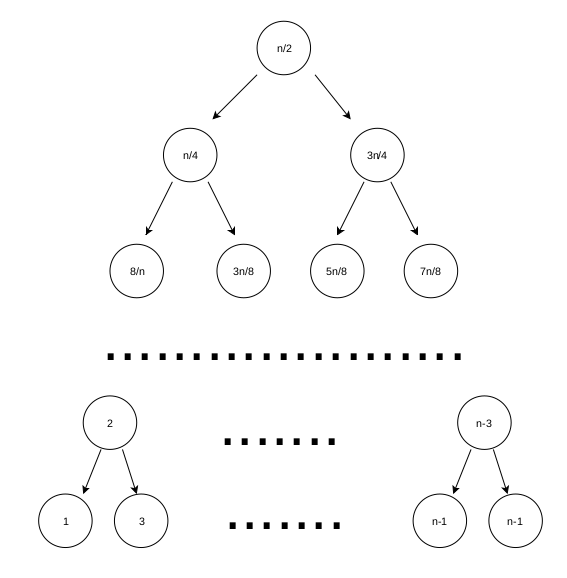
\includegraphics[scale = 0.4]{tree.png}
    \centering
\end{figure}

\textit{Proof:} From the proof in previous question, $i(k) \leq i(k+1)$. Find the middle point
of n, and find i($\frac{n}{2}$) at that point. Each recursive would have 2 times the elements
as the previous one. However, each one only need to do half the work, since the boundary is halved
on each recursion. Each level still does the same work. And we guarantee that every node is
found through the recursive call except $c_n$ and $c_0$. Therefore, determine the base case that find $c_{n-1}$
and find an extra $c_n$ using $c_{n-1}$ and extra $c_0$ using $c_1$.
\end{enumerate}
\end{document}